\chapter{Reti di Petri}
\section{Introduzione}
Le reti di Petri sono un modello formale per la descrizione di sistemi
distribuiti a tempo discreto. A differenza delle algebre di processo, come il CCS,
le reti di Petri permettono di descrivere la true concurrency di un
sistema concorrente, usando una semantica a ordine parziale.
A differenza del CCS, che analizza lo stato globale del sistema concorrente,
le reti di Petri permettono di rappresentare l'evoluzione degli stati
delle singole parti che compongono il sistema, senza dover esplicitamente
trattare lo stato globale del sistema concorrente (che molto spesso è
sconosciuto).\\
Le reti di Petri sono utili per verificare le proprietà di un sistema concorrente,
come liveness e assenza di deadlock, in modo da dimostrarne la correttezza.
Alcuni problemi di decisione su reti di Petri sono stati studiati da
Esparza e Nielsen (1995) METTERE CITAZIONE.

\section{Reti, eventi e grafi dei casi}
Le reti di Petri sono sistemi a transizione di stati che estendono la
classe delle reti elementari.
\begin{defn}
    Una \textbf{rete} è
\end{defn}

\begin{defn}
    Una \textbf{rete elementare} è
\end{defn}

\begin{defn}
    Una \textbf{rete di Petri} è una quadrupla $N = (P, T, F, m_0, W)$ tale che:
    \begin{itemize}
        \item $P$ è un insieme finito di \textbf{posti}
        \footnote{Con posto si intende lo stato di una parte del sistema
        che si vuole rappresentare. Lo stato globale farà invece riferimento a
        tutto il sistema.}.\\
        Un posto può essere visto come una condizione sul sistema che
        si vuole rappresentare.
        \item $T$ è un insieme finito di \textbf{transizioni}, dette anche
        eventi.
        \item $F \subseteq (B\times E)\cup(E\times B)$
        è una \textbf{relazione di flusso}, ovvero un insieme di
        archi diretti che collegano i posti alle transizioni e le transizioni
        ai posti. Gli archi non possono essere definiti tra posti e tra
        transizioni
        \footnote{Si può osservare che una rete definisce un grafo bipartito,
        dove i due sottoinsiemi che definiscono la partizione sono $P$ ed $T$.}.
        Per definizione, inoltre, ogni evento della rete ha almeno uno stato
        locale di ingresso e almeno uno stato locale di uscita.
        \[
            \forall e \in E, \exists p, q \in B : (p, e) \in F \land
            (e, q) \in F.
        \]
        \item $m_0$ è la marcatura iniziale della rete, che specifica quanti
        token sono presenti in ogni posto della rete di Petri.
        \item $W: F \rightarrow \mathbb{Z}$ è una funzione che assegna a ogni
        arco della rete un peso, rappresentante la sua molteplicità.
    \end{itemize}
\end{defn}
Senza perdere di generalità, si possono considerare le sole reti di Petri
in cui la funzione $W$ assegna a ogni arco della rete un peso pari a 1,
e in cui ogni posto ha una capacità di token massima pari a 1.
In questo caso, inoltre, la marcatura della rete di Petri collassa a una semplice
configurazione, ovvero a un sottoinsieme di posti della rete.
D'ora in poi verranno trattate solo reti di Petri di questo tipo, in modo
da semplificarne la trattazione.

Graficamente, gli elementi di una rete di Petri sono rappresentati come:
\begin{itemize}
    \item stato locale falso: $\fPlace$
    \item stato locale vero: $\tPlace$
    \item evento: $\event$
    \item transizione: $\longrightarrow$
\end{itemize}

\begin{defn}
    Dato un elemento $x \in B \cup E$, è possibile definire i due seguenti
    insiemi:
    \begin{align*}
        \preCond{x} &= \cbra{y \in B \cup E : (y, x) \in F}\\
        \postCond{x} &= \cbra{y \in B \cup E : (x, y) \in F}
    \end{align*}
    Se $x$ è un evento, allora $\preCond{x}$ sono le \textbf{pre-condizioni} di
    $x$, mentre $\postCond{x}$ sono le \textbf{post-condizioni} di $x$.\\
    Se invece $x$ è uno stato locale, $\preCond{x}$ sono i \textbf{pre-eventi}
    di $x$, mentre $\postCond{x}$ sono i \textbf{post-eventi} di $x$.

    \upperAccE possibile estendere la definizione di questi due insiemi anche
    a insiemi di stati locali ed eventi. Sia $X \subseteq B \cup E$, allora:
    \begin{align*}
        \preCond{X} &= \bigcup\limits_{x \in X} \preCond{x}\\
        \postCond{X} &= \bigcup\limits_{x \in X} \postCond{x}
    \end{align*}
\end{defn}

\begin{defn}
    Una rete di Petri è \textbf{semplice} sse:
    \[
        \forall x, y \in B \cup E, \preCond{x} = \preCond{y} \land
        \postCond{x} = \postCond{y} \rightarrow x = y
    \]
    \begin{marginfigure}[-5cm]
        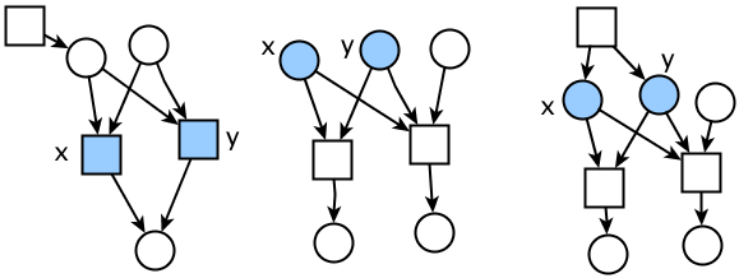
\includegraphics[width=1\linewidth]{img/reti_non_semplici.png}
        \caption{Reti non semplici}
        \label{fig:reti_non_semplici}
    \end{marginfigure}
\end{defn}

\begin{defn}
    Una rete di Petri è \textbf{pura} sse:
    \[
        \forall e \in E, \preCond{e} \cap \postCond{e} = \emptyset
    \]
    \begin{marginfigure}[-1cm]
        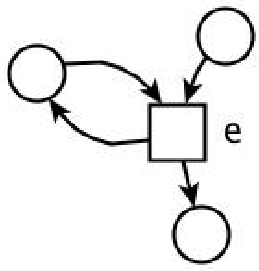
\includegraphics[width=0.4\linewidth]{img/rete_non_pura.png}
        \caption{Rete non pura.}
        \label{fig:rete_non_pura}
    \end{marginfigure}
\end{defn}

\begin{defn}
    Un evento $e$ è \textbf{abilitato} in una rete $N$ per la configurazione
    corrente $c$ sse:
    \[
        \preCond{e} \subseteq c \land \postCond{e} \cap c = \emptyset
    \]
    ovvero tutte le sue pre-condizioni sono vere, mentre tutte le sue
    post-condizioni sono false.\\
    La configurazione del sistema dopo aver eseguito $e$, indicata con $c'$,
    sarà:
    \[
        c' = \bra{c \setminus \preCond{e}} \cup \postCond{e}
    \]
    L'occorrenza di un evento $e$ nella configurazione corrente $c$ che porta
    alla configurazione $c'$ viene indicata con $\canFire{c}{e}{c'}$.
\end{defn}

\begin{defn}
    Un insieme di eventi $U \subseteq T$ è un \textbf{passo} sse tutti i suoi
    eventi sono indipendenti, ovvero eventi diversi di $U$ non condividono
    alcuno stato locale.
    \[
        \forall e_1, e_2 \in U, e_1 \neq e_2 \rightarrow
        (\preCond{e_1} \cup \postCond{e_1}) \cap
        (\preCond{e_2} \cup \postCond{e_2}) = \emptyset
    \]
\end{defn}

\begin{defn}
    Un insieme di eventi $U \subseteq T$ è un \textbf{passo abilitato}
    per la configurazione corrente $c$ sse:
    \[
        U \tn{ è un passo } \land \forall e \in U, \canFire{c}{e}{}
    \]
\end{defn}

\begin{defn}
    Siano $N_1 = (B_1, E_1, F_1)$ e $N_2 = (B_2, E_2, F_2)$ due sistemi
    elementari, $N_2$ è \textbf{sottorete} di $N_1$ sse:
    \begin{itemize}
        \item $B_2 \subseteq B_1$
        \item $E_2 \subseteq E_1$
        \item $F_2 = F_1 \cap \bra{\bra{B_2 \times E_2} \cup \bra{E_2 \times B_2}}$
    \end{itemize}
\end{defn}

\begin{defn}
    Sia $N = (B, E, F)$ una rete, la \textbf{sottorete generata da
    un sottoinsieme di stati locali} $B_1 \subseteq B$ è la rete
    $N_1 = (B_1, E_1, F_1)$ con:
    \begin{itemize}
        \item $E_1 = \preCond{B_1} \cup \postCond{B_1}$
        \item $F_1 = F \cap\bra{\bra{B_1 \times E_1} \cup \bra{E_1 \times B_1}}$
    \end{itemize}
\end{defn}

\begin{defn}
    Sia $N = (B, E, F)$ una rete, la \textbf{sottorete generata da un
    sottoinsieme di eventi} $E_1 \subseteq E$ è la rete
    $N_1 = (B_1, E_1, F_1)$ con:
    \begin{itemize}
        \item $B_1 = \preCond{E_1} \cup \postCond{E_1}$
        \item
        $F_1 = F \cap \bra{\bra{B_1 \times E_1} \cup \bra{E_1 \times B_1}}$
    \end{itemize}
\end{defn}

\subsection*{Grafo dei casi e grafo dei casi sequenziale}
\begin{defn}
    L'\textbf{insieme delle configurazioni raggiungibili}
    $C_{\Sigma} \subseteq 2^{B}$ nella rete di Petri $(P, T, F, c_{\tn{start}})$
    è definito come:
    \begin{itemize}
        \item $c_{\tn{start}} \in C_{\Sigma}$
        \item $\bra{c \in C_{\Sigma} \land \exists U \subseteq T :
        \canFire{c}{U}{c'}} \rightarrow c' \in C_{\Sigma}$
    \end{itemize}
\end{defn}

\begin{defn}
    L'\textbf{insieme dei passi} $U_{\Sigma}$ di un sistema elementare $\Sigma$
    sono tutti i passi possibili che il sistema $\Sigma$ può compiere.
    \[
        U_{\Sigma} = \cbra{U \subseteq E \, | \,
        \exists c_1, c_2 \in C_{\Sigma} : \canFire{c_1}{U}{c_2}}
    \]
\end{defn}

Il comportamento di una rete di Petri
può essere descritto completamente con un grafo dei casi, in cui ogni nodo
rappresenta una delle possibili configurazioni raggiungibili della rete
e ogni arco $(c_i, c_j)$ etichettato con $U$ rappresenta l'esecuzione
$\canFire{c_i}{U}{c_j}$ di un passo abilitato $U$ per $c_i$.
Essendo un arco etichettato con un passo abilitato del sistema, il grafo
dei casi $CG_{\Sigma}$ descrive la \textbf{step semantics} del sistema
considerato.

\begin{defn}
    Il \textbf{grafo dei casi} $CG_{\Sigma}$ di una rete di Petri $\Sigma$ è
    formalmente definito come la quadrupla
    $(C_{\Sigma}, U_{\Sigma}, A, c_{\tn{start}})$ dove:
    \begin{itemize}
        \item $C_{\Sigma}$, l'insieme dei casi raggiungibili, è l'insieme
        dei nodi.
        \item $U_{\Sigma}$, l'insieme dei passi, è l'alfabeto del grafo.
        \item $A = \cbra{(c, U, c') \, | \, c, c' \in C_{\Sigma} \land
        U \in U_{\Sigma} \land \canFire{c}{U}{c'}}$
        è l'insieme degli archi
        \footnote{Ogni arco è quindi etichettato con un \textit{passo},
        ovvero con un insieme di eventi del sistema $\Sigma$.}.
        \item $c_{\tn{start}}$ è la configurazione di partenza.
    \end{itemize}
\end{defn}

\begin{property}
    Il grafo dei casi gode della \textbf{diamond property}.\\
    Se un grafo dei casi $CG_{\Sigma}$ per un sistema elementare
    $\Sigma = (C_{\Sigma}, U_{\Sigma}, A, c_{\tn{start}})$ presenta gli archi
    $(c_1, U_1, c_2)$, $(c_2, U_2, c_3)$ e $(c_1, U_2, c_4)$, con
    $c_1, c_2, c_3, c_4 \in C_{\Sigma} \land U_1, U_2 \in U_{\Sigma} \land
    U_1 \cap U_2 = \emptyset$,\\
    allora sicuramente il sistema $\Sigma$ ammetterà i passi
    $(c_4, U_1, c_3)$ e $(c_1, U_1 \cup U_2, c_3)$.
    \begin{marginfigure}[1cm]
        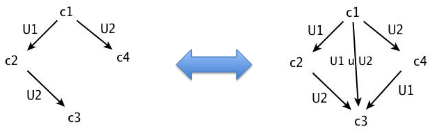
\includegraphics[width=1.05\linewidth]{img/diamond_property.png}
        \caption{Diamond property.}
        \label{fig:diamond_property}
    \end{marginfigure}
\end{property}
Gli archi del grafo dei casi sono etichettati
con un \textit{sottoinsieme} di eventi concorrenti che possono scattare dalla
configurazione di partenza. Questa semantica, come già detto, prende il nome di
step semantic.
Se però si è interessati a descrivere il comportamento del sistema concorrente
preso in analisi analizzando le possibili sequenze di eventi
che sono possibili al suo interno, senza interessarsi a quali eventi
possono essere eseguiti in maniera concorrente, allora è possibile definire
un grafo dei casi sequenziale. Il grafo dei casi sequenziale si differenzia
dal grafo dei casi solo per il fatto che i suoi archi sono etichettati con un
\textit{singolo evento}, senza quindi esplicitare un insieme di eventi
eseguibili concorrentemente.
La semantica descritta dal grafo dei casi sequenziale prende il nome
di semantica a \textbf{interleaving}, e altro non è
che una simulazione sequenziale non deterministica del sistema.

Il grafo dei casi sequenziale, inoltre, è, di fatto, un sistema a transizioni
etichettato che modella il sistema concorrente preso in analisi,
e può quindi essere usato per verificare alcune proprietà del sistema
concorrente che si sta analizzando.
Data una rete di Petri, però, trovare l'insieme delle configurazioni raggiungibili
può essere complesso e portare a un'esplosione combinatoria:
per verificare proprietà su un sistema concorrente, quindi, spesso
si preferisce ridursi a sottocasi di reti di Petri più facili da gestire,
o si preferiscono altri metodi formali, come le logiche temporali.

\begin{defn}
    Il \textbf{grafo dei casi sequenziale} $SCG_{\Sigma}$ di una rete
    di Petri $\Sigma$ è una quadrapla $(C_{\Sigma}, E, A, c_{\tn{start}})$
    dove:
    \begin{itemize}
        \item $C_{\Sigma}$, l'insieme dei casi raggiungibili, è l'insieme dei
        nodi.
        \item $E$, l'insieme degli eventi, è l'alfabeto del grafo con cui
        verranno etichettati gli archi.
        \item $A = \cbra{(c, e, c') \, | \, c, c' \in C_{\Sigma} \land
        e \in E \land \canFire{c}{e}{c'}}$
        è l'insieme degli archi.
        \item $c_{\tn{start}}$ è la configurazione di partenza.
    \end{itemize}
\end{defn}

\begin{marginfigure}
    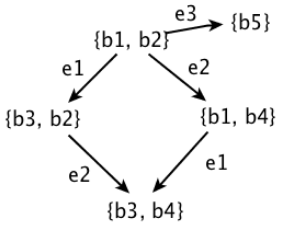
\includegraphics[width=0.60\linewidth]{img/grafo_casi_sequenziale.png}
    \caption{Grafo dei casi sequenziale.}
    \label{fig:sequential_case_graph}
\end{marginfigure}

\begin{property}
    Il grafo dei casi $CG_{\Sigma}$ e il grafo dei casi sequenziale
    $SCG_{\Sigma}$ della stessa rete di Petri $\Sigma$ sono
    \textbf{sintatticamente equivalenti}, ovvero è possibile ottenere uno a
    partire dall'altro usando solo procedimenti di modifica sintattica.
\end{property}

\begin{rem}
    Il grafo dei casi è un sistema di transizioni etichettato per il sistema
    concorrente descritto dalla rete.
    Trovare quindi un sistema di transizioni etichettato che esprime il
    comportamento del sistema è molto semplice: esso coincide infatti con
    il grafo dei casi.
    Trovare invece una rete elementare con grafo dei casi isomorfo a un
    sistema di transizioni etichettato dato risulta più complicato,
    e prende il nome di problema della sintesi. Esso viene risolto con la
    teoria delle regioni.
\end{rem}

\subsection*{Equivalenza semantica tra reti di Petri}
    Due reti di Petri $\Sigma_1$ e $\Sigma_2$ sono equivalenti sse
    i loro grafi dei casi (e di conseguenza anche i loro grafi dei casi
    sequenziali, in quanto sintatticamente equivalenti) sono isomorfi, ovvero
    $\exists \alpha: S_1 \rightarrow S_2 \land \exists \beta: E_1 \rightarrow E_2$
    funzioni biunivoche tali che DA SISTEMARE LE LETTERE:
    \begin{itemize}
        \item $\alpha(s_1) = s_2$, ovvero la configurazione di partenza di
        $S_1$ viene mappata nella configurazione di partenza di $S_2$;
        \item $\forall s_i, s_j \in S_1 \land \forall e \in E_1, \quad
        (s_i, e, s_j) \in T_1 \leftrightarrow (\alpha(s_i), \beta(e), \alpha(s_j)) \in T_2$.
    \end{itemize}

\section{Situazioni particolari}
\subsection*{Contatto}
\begin{defn}
    Siano $\Sigma = (B, E, F, c_{\tn{start}})$ un sistema elementare, $e \in E$
    un evento e $c \in C_{\Sigma}$ una possibile configurazione di $\Sigma$,
    $(e, c)$ è un \textbf{contatto} sse:
    \[
        \preCond{e} \subseteq c \land \postCond{e} \cap c \neq \emptyset
    \]
    ovvero tutte le pre-condizioni di $e$ sono vere, ma almeno una
    post-condizione di $e$ è vera.\\
    Un evento che si trova in uno stato di contatto non è abilitato.
\end{defn}

\begin{rem}
    Un evento senza precondizioni è sicuramente un contatto: viene infatti
    eseguito subito, in quanto l'insieme vuoto delle precondizioni è sempre
    vero, e quindi le post-condizioni diventano vere. Ma poi l'evento, non
    avendo pre-condizioni, avrà sicuramente le pre-condizioni vere e tutte
    le post-condizioni vere. Di conseguenza si ha un contatto.
\end{rem}

\begin{defn}
    Un sistema elementare $\Sigma = (B, E, F, c_{\tn{start}})$ è un
    \textbf{sistema senza contatti} sse:
    \[
        \forall e \in E, \forall c \in C_{\Sigma} \quad
        \preCond{e} \subseteq c \rightarrow \postCond{e} \cap c = \emptyset
    \]
    ovvero se, qualunque sia la configurazione del sistema, le pre-condizione
    di un evento sono vere, allora sicuramente tutte le sue post-condizioni
    sono false, e l'evento è abilitato \footnote{In un sistema elementare
    senza contatti, per stabilire se un evento è abilitato non è necessario
    effettuare alcun controllo sulle post-condizioni: se le pre-condizioni
    sono vere, infatti, le post-condizioni saranno sicuramente false.}.
\end{defn}

\begin{rem}
    Ogni sistema elementare $\Sigma$ con contatti può essere trasformato in un
    sistema elementare $\Sigma'$ senza contatti e con grafo dei casi isomorfo.\\
    Per farlo, per ogni stato $s$ che può essere contatto deve essere aggiunto
    uno stato complementare $\overline{s}$, vero solo quando $s$ è falso.
\end{rem}

\begin{marginfigure}[-10cm]
    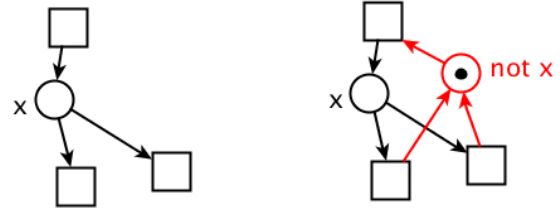
\includegraphics[width=1\linewidth]{img/contatto_complementare.png}
    \caption{Rimozione di un contatto tramite l'aggiunta dello stato complementare.}
    \label{fig:sistema_con_contatti}
\end{marginfigure}

\subsection*{Conflitto}
\begin{defn}
    Siano $\Sigma = (B, E, F, c_{\tn{start}})$ un sistema elementare,
    $e_1, e_2 \in E$ due evento e $c \in C_{\Sigma}$ una possibile
    configurazione di $\Sigma$, $e_1$ ed $e_2$ sono in \textbf{conflitto}
    in $c$ sse:
    \[
        \canFire{c}{e_1}{} \land \canFire{c}{e_2}{} \land
        \lnot \canFire{c}{\cbra{e_1, e_2}}{}
    \]
    ovvero entrambi gli eventi sono abilitati, ma il verificarsi di uno rende
    l'altro non abilitato. Di conseguenza, i due eventi non possono essere
    eseguiti in maniera concorrente. Non sapendo quale dei due eventi verrà
    effettivamente eseguito, un conflitto esprime non determinismo.

    Esistono due tipi di conflitti:
    \begin{itemize}
        \item in avanti: due eventi abilitati hanno la stessa pre-condizione.
        Il verificarsi di un evento rende falsa la pre-condizione in comune,
        disabilitando l'altro evento;
        \item all'indietro: due eventi abilitati hanno la stessa
        post-condizione. Il verificarsi di un evento rende vera la
        post-condizione in comune, disabilitando l'altro evento.
    \end{itemize}

    \begin{marginfigure}[-11cm]
        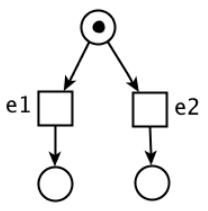
\includegraphics[width=0.75\linewidth]{img/conflitto_avanti.png}
    \caption{Conflitto in avanti.}
    \label{fig:conflitto_avanti}
    \end{marginfigure}

    \begin{marginfigure}[-3cm]
        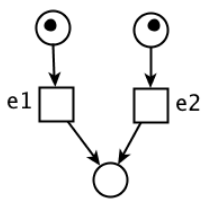
\includegraphics[width=0.75\linewidth]{img/conflitto_indietro.png}
        \caption{Conflitto all'indietro.}
        \label{fig:conflitto_indietro}
    \end{marginfigure}
\end{defn}

\subsection*{Confusione}
La confusione si presenta in un sistema con conflitti in cui la struttura non
permette di stabilire se, nel passaggio da una configurazione $c$ a una
configurazione $c'$, è stato risolto un conflitto.

\begin{figure}
    \centering
    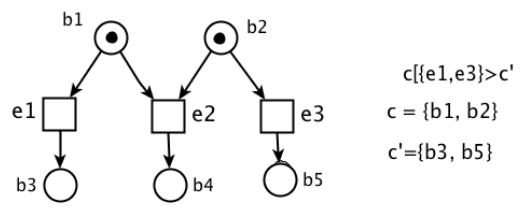
\includegraphics[width=0.5\linewidth]{img/confusione.png}
    \label{fig:confusione}
\end{figure}
In questo sistema non è possibile stabilire se, passando da $c$ a $c'$, sia
stato risolto un conflitto tra $e_1$ ed $e_2$ o tra $e_2$ ed $e_3$.

Un altro esempio di confusione si verifica nella mutua esclusione.

\subsection*{Sequenza}
Siano $\Sigma = (B, E, F, c_{\tn{start}})$ un sistema elementare,
$e_1, e_2 \in E$ due eventi e $c \in C_{\Sigma}$ una possibile configurazione
di $\Sigma$, $e_1$ ed $e_2$ sono in \textbf{sequenza} in $c$ sse:
\[
    \canFire{c}{e_1}{} \land \lnot \canFire{c}{e_2}{} \land
    \canFire{\canFire{c}{e_1}{c'}}{e_2}
\]
ovvero $e_2$ può essere eseguito sse prima viene eseguito $e_1$.
C'è quindi una dipendenza causale tra gli eventi $e_1$ ed $e_2$.

\begin{figure}
    \centering
    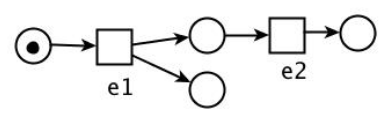
\includegraphics[width=0.5\linewidth]{img/sequenza.png}
    \caption{Due eventi in sequenza.}
    \label{fig:eventi_sequenza}
\end{figure}

\subsection*{Concorrenza}
Siano $\Sigma = (B, E, F, c_{\tn{start}})$ un sistema elementare,
$e_1, e_2 \in E$ due eventi e $c \in C_{\Sigma}$ una possibile configurazione
di $\Sigma$, $e_1$ ed $e_2$ sono \textbf{concorrenti} in $c$ sse:
\[
    \canFire{c}{\cbra{e_1, e_2}}{}
\]
ovvero $\cbra{e_1, e_2}$ è un passo abilitato. Questo significa che i due
eventi $e_1$ ed $e_2$ sono indipendenti ed entrambi abilitati in $c$.

\begin{figure}
    \centering
    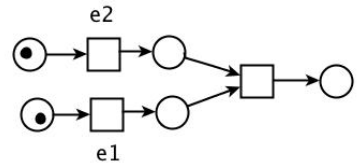
\includegraphics[width=0.5\linewidth]{img/eventi_concorrenti.png}
    \caption{Due eventi concorrenti.}
    \label{fig:eventi_concorrenti}
\end{figure}

\section{Processi non sequenziali e processi ramificati}
Prima di poter spiegare cosa sono i processi non sequenziali e i processi
ramificati, è necessario introdurre alcune nozioni.

\subsection*{Relazioni sugli elementi di una rete}
\begin{defn}
    La relazione d'ordine parziale largo \footnote{Una relazione d'ordine largo
    è una relazione riflessiva, antisimmetrica e transitiva.}
    $\le \, \subseteq (B \cup E) \times (B \cup E)$ specifica se un elemento
    è causa di un altro elemento, ed è definita come:
    \[
        \forall x, y \in B \cup E, \quad (x, y) \in \, \le \quad
        \tn{ sse } \quad x F^*y
    \]
    ovvero è possibile raggiungere $y$ a partire da $x$ usando un numero
    limitato di transizioni. Se $(x,y) \in \, \le$, allora $x$ causa $y$.
    Si può notare che, in questa relazione, un elemento $x$ causa sè stesso.
\end{defn}

\begin{defn}
    La relazione d'ordine parziale stretto \footnote{Una relazione d'ordine
    stretto è una relazione irriflessiva, asimmetrica e transitiva.}
    $< \, \subseteq (B \cup E) \times (B \cup E)$ specifica se un elemento
    è causa di un altro elemento diverso da sè stesso, ed è definita come:
    \[
        \forall x, y \in B \cup E, \quad (x, y) \in \, < \quad \tn{ sse } \quad
        x F^*y \land x \neq y
    \]
\end{defn}

\begin{rem}
    $<$ è facilmente ottenibile da $\le$ rimuovendo tutte le coppie della forma
    $(x,x), \forall x \in B \cup E$.
\end{rem}

\begin{defn}
    Sia $N$ una rete di Petri, la \textbf{relazione di conflitto}
    $\# \subseteq P \cup T$ specifica quali coppie di elementi della rete $N$
    sono causalmente dipendenti da un conflitto in avanti, ed è definita come:
    \[
        x \# y \quad \tn{ sse } \quad \exists e_1, e_2 \in E,
        (e_1 \neq e_2 \land e_1 \le x \land e_2 \le y) :
        \preCond{e_1} \cap \preCond{e_2} \neq \emptyset
    \]
\end{defn}

\begin{rem}
    La relazione di conflitto $\#$ è simmetrica ma non transitiva.
\end{rem}

\begin{defn}
    La relazione $\tn{li} \subseteq (B \cup E) \times (B \cup E)$ specifica
    quali elementi della rete sono causalmente dipendenti, ed è definita come:
    \[
        \forall x, y \in B \cup E, \quad (x, y) \in \tn{ li} \quad
        \tn{ sse } \quad (x,y) \in \, \le \lor \, (y,x) \in \, \le
    \]
\end{defn}

\begin{defn}
    La relazione $\tn{co} \subseteq (B \cup E) \times (B \cup E)$ specifica
    quali elementi della rete sono causalmente indipendenti, ed è definita come:
    \[
        \forall x, y \in B \cup E, \quad (x, y) \in \tn{ co} \quad \tn{ sse } \quad
        (x,y) \notin \, < \land \, (y,x) \notin \, < \land \, (x,y) \notin \#
    \]
\end{defn}

\begin{rem}
    \begin{align*}
        (x,y) \in \tn{ li } &\longleftrightarrow (y,x) \in \tn{ li}\\
        (x,y) \in \tn{ co } &\longleftrightarrow (y,x) \in \tn{ co}
    \end{align*}
\end{rem}
\begin{rem}
    $\tn{li}$ e $\tn{co}$ sono relazioni riflessive, simmetriche ma non
    transitive.
\end{rem}

\subsection*{Tagli e linee}
\begin{defn}
    Un \textbf{coset} $C \subseteq P \cup T$ è un insieme di elementi
    della rete di Petri tale che:
    \[
        \forall x, y \in C, x \tn{ co } y
    \]
    ovvero gli elementi di un coset sono tutti causalmente indipendenti tra
    loro.
\end{defn}

\begin{rem}
    In un coset, la relazione $\tn{co}$ è transitiva.
\end{rem}

\begin{defn}
    Un \textbf{taglio} $C \subseteq P \cup T$ è un coset massimale, ovvero:
    \[
        C \tn{ è un coset } \, \land \, \forall x \in (B \cup E) \setminus C, \,
        \exists c \in C : x \tn{ li } c
    \]
    ovvero ogni altro elemento che non appartiene a $C$ è causalmente
    dipendente da almeno un elemento di $C$, o viceversa.
\end{defn}

\begin{defn}
    Un taglio $C$ è un \textbf{P-taglio} sse $C \subseteq P$, ovvero è formato
    da soli stati locali.
\end{defn}

\begin{rem}
    Un P-taglio corrisponde a uno dei possibili casi raggiungibili della rete.
    Di conseguenza, tutti i possibili P-tagli definiscono tutti i possibili
    casi raggiungibili della rete.
\end{rem}

\begin{defn}
    Un taglio $C$ è un \textbf{T-taglio} sse $C \subseteq T$, ovvero è formato
    da soli eventi.
\end{defn}

\begin{rem}
    Tutti gli eventi all'interno di un T-taglio possono essere eseguiti in
    maniera concorrente. Essendo un T-taglio l'insieme di cardinalità massima
    $n$ che contiene solo eventi indipendenti tra loro, il sistema necessita
    di $n$ processori per l'esecuzione in minor tempo possibile degli $n$
    eventi.\\
    Il numero di processori per una rete (da cui si deriva la rete di
    occorrenze), è pari alla cardinalità massima tra le cardinalità degli
    T-tagli di tutti i processi non sequenziale che è possibile definire.
\end{rem}

\begin{defn}
    Un \textbf{liset} $L \subseteq P \cup T$ è un insieme di elementi della
    rete di Petri tale che:
    \[
        \forall x, y \in L, x \tn{ li } y
    \]
    ovvero gli elementi di un liset sono tutti causalmente dipendenti tra loro.
\end{defn}

\begin{rem}
    In un liset, la relazione $\tn{li}$ è transitiva.
\end{rem}

\begin{defn}
    Una \textbf{linea} $L \subseteq P \cup T$ è un liset massimale, ovvero:
    \[
        L \tn{ è un coset } \, \land \, \forall x \in (B \cup E) \setminus L, \,
        \exists l \in L : x \tn{ co } l
    \]
    ovvero ogni altro elemento che non appartiene a $L$ è causalmente
    indipendente da almeno un elemento di $C$, o viceversa.
\end{defn}

\subsection*{Processo ramificato}
\begin{defn}
    Una rete di Petri è una \textbf{rete di occorrenze} sse:
    \begin{itemize}
        \item $\forall p \in P, |\preCond{p}| = 1$, ovvero non sono
        accettati conflitti all'indietro. Sono invece accettati
        i conflitti in avanti.
        \item $\forall x, y \in P \cup T, (x,y) \in F^+ \rightarrow
        (y,x) \notin F^+$, ovvero non sono presenti cicli.
        \item $\forall e \in T$, l'insieme $\cbra{x \in P \cup T : x F^*e}$,
        ovvero il passato di ogni evento, ha cardinalità finita.
        \item la relazione di conflitto $\#$ è irriflessiva \footnote{E di
        conseguenza antisimmetrica.}, ovvero un unico elemento non dipende
        causalmente da due eventi in conflitto in avanti.
    \end{itemize}
\end{defn}

Su una rete di occorrenze è possibile definire le funzioni
\begin{align*}
    \tn{past}: P \cup T &\rightarrow \mathcal{P}(P \cup T)\\
    \tn{future}: P \cup T &\rightarrow \mathcal{P}(P \cup T)
\end{align*}

$\tn{past}$ restituisce tutti gli elementi della rete che causano $x$, mentre
$\tn{future}$ restituisce tutti gli elementi che sono causati da $x$.\\
Per definizione di rete di occorrenze, $\tn{past}(x)$ è sicuramente un insieme
di cardinalità finita, mentre $\tn{past}(x)$ può avere cardinalità infinita
numerabile.

\begin{rem}
    Tutti gli elementi della rete che non appartengono nè a $\tn{past}(x)$ nè
    a $\tn{future}(x)$ possono essere eseguiti in maniera concorrente rispetto
    a $x$.
\end{rem}

\begin{defn}
    Un \textbf{processo ramificato} di una rete di Petri $N_1 = (P_1, T_1, F_1, c_1)$
    senza contatti e finita (e quindi $k$-densa), è una coppia
    $(N_2, \phi), N_2 = (P_2, T_2, F_2, c_2)$ tale che:
    \begin{itemize}
        \item $N_2$ è una rete di occorrenze;
        \item $\phi: P_2 \cup T_2 \rightarrow P_1 \cup T_1$ è una funzione
        tale che:
        \begin{itemize}
            \item $\phi(P_2) \subseteq P_1 \land \phi(T_2) \subseteq T_1$
            \item $\forall e_1, e_2 \in T_2, \, (\preCond{e_1} = \preCond{e_2}
            \land \phi(e_1) = \phi(e_2)) \implies e_1 = e_2$
            \item FINIRE DEFINIZIONE
        \end{itemize}
    \end{itemize}
\end{defn}

\begin{rem}
    Un processo ramificato contiene una o più run della rete di Petri da cui
    è stato costruito.
\end{rem}

\subsection*{Processo non sequenziale}
Una rete causale è un tipo particolare di rete di occorrenze, che non presenta
alcun conflitto.\\
Una \textbf{rete causale} è una rete di Petri tale che
\footnote[][-1cm]{L'ulteriore condizione presente nelle reti di occorrenza,
ovvero che la relazione di conflitto sia irriflessiva, collassa nella prima
condizione per le reti clausali: non avendo alcun conflitto, per la rete
clausale vale $\# = \emptyset$.}:
\begin{itemize}
    \item $\forall b \in B, \lvert \preCond{b} \rvert \le 1 \land \lvert \postCond{b} \rvert \le 1$,
    ovvero non sono presenti conflitti \footnote[][1cm]{In un conflitto in
    avanti, lo stato pre-condizione ha due post-eventi. In un conflitto
    all'indietro, lo stato post-condizione ha due pre-eventi. Di conseguenza,
    imporre un numero di pre-eventi e post-eventi minore o uguale a uno implica
    l'assenza di conflitti.};
    \item $\forall x, y \in B \cup E, \quad (x, y) \in F^+ \rightarrow (y, x) \notin F^+$,
    ovvero non sono presenti cicli;
    \item $\forall e \in E$, la cardinalità dell'insieme $\cbra{x \in B \cup E | x \, F^* e}$
    è finita, ovvero i predecessori di un qualsiasi evento sono in numero
    finito.
\end{itemize}

\begin{rem}
    Una rete causale ammette elementi isolati, ovvero elementi senza archi
    in ingresso e archi in uscita.
\end{rem}

Una rete causale rappresenta una sola delle possibili esecuzioni del sistema
concorrente, ovvero un suo processo non sequenziale.
La coppia $(N, \phi)$ che definisce un processo non sequenziale
è quindi il processo non sequenziale costruito dalla rete $N$ usando la
funzione $\phi$. Diversi processi non sequenziali per la stessa rete
definiranno la funzione $\phi$ in maniera diversa ($\phi$ deve comunque
rispettare tutte le caratteristiche che deve avere la funzione che permette
di definire un processo non sequenziale).

\begin{defn}
    Un \textbf{processo non sequenziale} di una rete di Petri $N_1$
    senza contatti e finita (e quindi $k$-densa) è una coppia $(N_2, \phi)$
    tale che:
    \begin{itemize}
        \item $N_2$ è una rete causale;
        \item $\phi: B \cup E \rightarrow S \cup T$ è una funzione tale che
        FINIRE DEFINIZIONE
    \end{itemize}
\end{defn}

\begin{defn}
    Una rete è \textbf{\textit{k}-densa} se ogni linea si interseca una singola
    volta con ogni altro taglio e, viceversa, ogni taglio si interseca una
    singola volta con ogni altra linea.
\end{defn}

Un taglio e una linea si intersecano esattamente in un punto perchè se si
incontrassero in più punti, allora tutti i punti di intersezione
rappresenterebbero elementi che sono contemporaneamente casualmente
dipendenti (li) e casualmente indipendenti (co), violando quindi i tagli
e le linee definite.

\begin{rem}
    Una rete finita è sicuramente $k$-densa.
\end{rem}

\subsection*{Prefisso e unfolding}
\begin{defn}
    Sia $\Sigma = (S, T , F , c_in)$ un sistema elementare finito e senza contatti
    e siano $\Pi_1 = (N_1, \phi_1)$, $\Pi_2 = (N_2, \phi_2)$ due suoi processi
    ramificati.
    $\Pi_1$ è un prefisso di $\Pi_2$ sse:
    \begin{itemize}
        \item $N_1$ è una sottorete di $N_2$
        \item $\phi_2|N_1 = \phi_1$, ovvero $\phi_2$ ”ristretto” a $N_1$ è
        uguale a $\phi_1$.
    \end{itemize}
\end{defn}

\begin{defn}
    L'\textbf{unfolding} di una rete elementare $\Sigma$ è il processo ramificato
    massimale, ovvero il processo ramificato che include tutte le possibili
    run di $\Sigma$.
\end{defn}

\begin{rem}
    Ogni processo ramificato (compresi i processi non sequenziali, in quanto
    sono casi particolari di processi ramificati con una singola run) è un
    prefisso dell'unfolding.
\end{rem}

è possibile anche cercare di individuare un prefisso finito dell'unfolding
che permetta di derivare tutte le possibili informazioni riguardo il comportamento
del sistema elementare. Questo prefisso prende il nome di prefisso completo.


\section{Estensioni}
AGGIUNGERE RETI COLORATE, DOVE TOKEN HANNO COLORE DIVERSO.
Fino ad ora sono state considerate solo reti elementari, ovvero reti di Petri
che tollerano al massimo un token per stato e che prevedono che ogni evento
sottragga un token da ogni precondizione, e aggiunga un token a ogni
precondizione.

è possibile però anche definire reti di Petri che tollerano più token
per ogni stato (ogni stato ha una certa capacità massima) e ogni evento
può richiedere che in una sua precondizione siano presenti più di un token.
Quando l'evento scatta verranno rimossi più token da una precondizione.
Stesso ragionamento può essere applicato alle post-condizioni, in cui l'evento
aggiunge più di un token.
In entrambi casi, il fatto che vengano usati più token viene specificato mettendo
un numerino vicino all'arco che collega l'evento alla pre-condizione o alla
post-condizione.

Queste reti di Petri più ad alto livello prendono il nome di reti Posti e Transizioni.
Reti elementari e reti Posti e Transizioni hanno la stessa capacità espressiva:
le reti Posti e Transizioni permettono semplicemente di definire una rete
più compatta, e quindi più facile da rappresentare.

Su una rete Posti e Transizioni in cui ogni stato ha capacità infinita
e non sono presenti cappi, allora è possibile definire una matrice di incidenza:
le righe corrispondono agli stati, mentre le colonne alle transizioni;
il peso degli archi sarà semplicemente il numero di token rimossi, se l'arco
va da precondizione a evento, o token aggiunti, se l'arco va da evento a
post-condizione.

La matrice di incidenza può essere usata per simulare le transizioni.
Sia infatti $M_i$ la configurazione corrente della rete, rappresentata come
una colonna "in più" della matrice in cui si associa a ogni stato il numero
di token, allora si può trovare la prossima configurazione della rete
allo scattare dell'evento $t$ semplicemente sommando la colonna associata
alla configurazione di partenza e la colonna associata a $t$.
La nuova colonna ottenuta è la nuova configurazione.

Si può affermare quindi che una configurazione $M_1$ è raggiungibile
da $M_0$ allo scattare di $t$, ovvero $M_0[t>M_1$ sse $M_0 + t = M_1$.
Questa equazione prende il nome di equazione di stato.

Sulle reti Posti e Transizioni con capacità infinita per ogni stato
possono essere definite delle proprietà:
\begin{itemize}
    \item la rete è limitata (bounded)  sse
    \item safe
    \item terminante sse non ammette sequenze infinite
    \item deadlock-free
    \item live sse
    \item reversibile/ciclico
    \item FINIRE
\end{itemize}

Queste proprietà possono essere verificate algoritmicamente (non visto durante
il corso).
